\documentclass[11pt, oneside]{article}   	% use "amsart" instead of "article" for AMSLaTeX format
\usepackage{geometry}                		% See geometry.pdf to learn the layout options. There are lots.
\geometry{letterpaper}                   		% ... or a4paper or a5paper or ... 
%\usepackage[parfill]{parskip}    		% Activate to begin paragraphs with an empty line rather than an indent
\usepackage{graphicx}				% Use pdf, png, jpg, or eps§ with pdflatex; use eps in DVI mode
								% TeX will automatically convert eps --> pdf in pdflatex		
\usepackage{mathtools}
\usepackage{hyperref}
\hypersetup{
    colorlinks=true,
    linkcolor=red,
    citecolor=magenta,      
    urlcolor=blue,
}
\urlstyle{same}
\usepackage{authblk}
\usepackage{float}

\usepackage{amssymb}

%SetFonts

\title{Automated Discovery of Temperature Dependent Structural Change\\
	\large SMC Data Challenge 2017}
\author[1]{Gabriel Santucci}
\affil[1]{Nucleon Decay and Neutrino Group, Stony Brook University Physics Department}
\date{August 2017}

\begin{document}
\maketitle


\begin{abstract}
	In this study we look for phase transitions as a function of temperature by inspecting data from neutron diffraction. A phase transition is defined here as a structural change in the analyzed  material. We characterize the intensity peak structure in the diffraction data at adjacent temperatures to conclude if a phase transition has occured.
\end{abstract}





\section{Introduction} \label{Intro}
	We are interested here in finding an algorithm to decide if a phase transition occurred in a material between two different temperatures. The data structure is given by different curves of Intensity (I) as a function of distance (d - characteristic spacing of the material in Angstroms) for different values of temperature (T).
To define a phase transition we first study one particular peak in the intensity curves, namely the peak between 3.2 and 3.3 ${\AA}$. The characterization of this peak consists of calculating its center, a characteristic width and the area under it.
Once we have the characterization procedure we move on  to characterize all the peaks in the data set for a given temperature value. Finally, one can define a phase transition by looking at the sets of peaks and its characteristics for two different adjacent curves (temperatures). We define a phase transition as a distinct change in structure of the intensity peaks.

\section{Inspecting the Data} \label{Data}
	Before we inspect any particular peaks, let us look at different sets of curves for randomly chosen values of temperatures to understand how the peak structure looks like. Figure \ref{fig:randTs}  shows the curves of intensity as a function of d-spacing for random values of temperature.

\begin{figure}[h]
  \centering
  %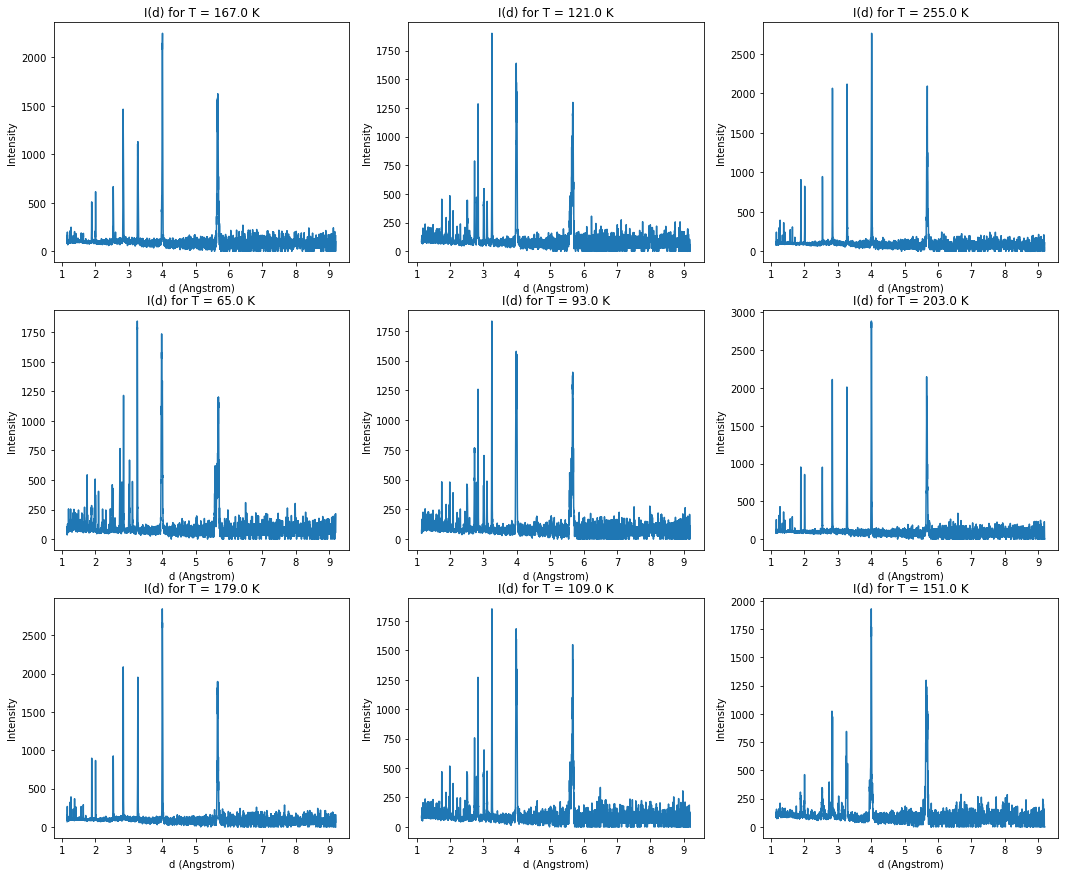
\includegraphics[scale=0.35, width=0.8\linewidth]{../figs/randomTs.png}
  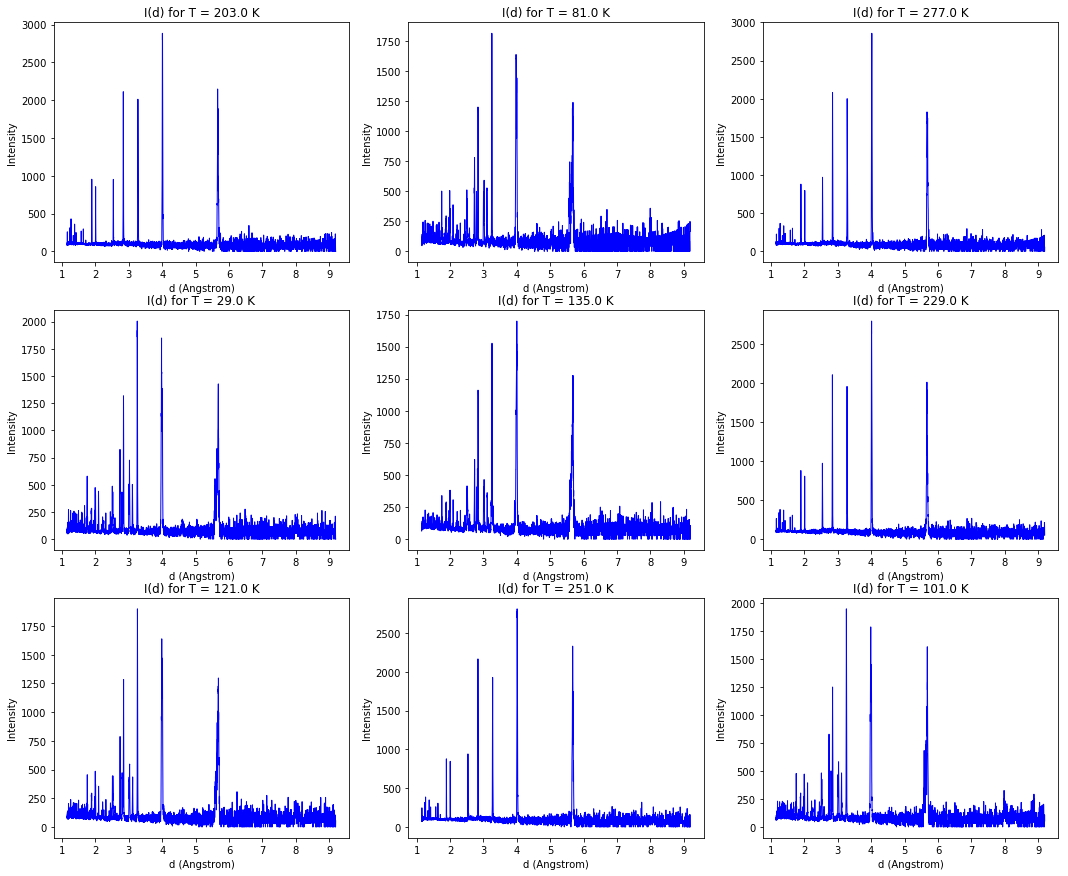
\includegraphics[scale=0.3]{../poster/figs/Icurves.png}
  \caption{Intensity curves as a function of d-spacing for different values of temperature.}
  \label{fig:randTs}
\end{figure}

We can also look at the maximum intensity distribution as a function of temperature. Figure \ref{fig:maxI} shows the highest value of I for each temperature T. We can already see a big hint of a structure change at around $\textrm{T} = 150 \textrm{ K}$. This particular data set has a unique maximum intensity value for each temperature. This allows us to uniquely map a temperature to an intensity value and vice-versa. So given a temperature value we can find the corresponding set of intensity values or the opposite.
This is certainly not a general result valid for any data set, but it is valid for the particular one that we are working with here. Building this one-to-one map makes it faster to get a curve given a temperature and also scales a lot faster with more data, in case the new data also presents this feature.

\begin{figure}[h]
  \centering
  %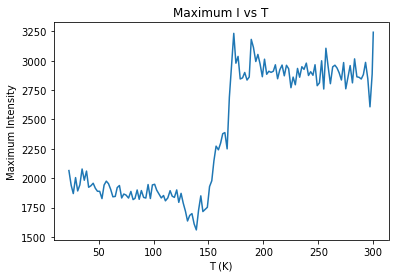
\includegraphics[scale=0.1, width=0.8\linewidth]{../figs/maxI.png}
  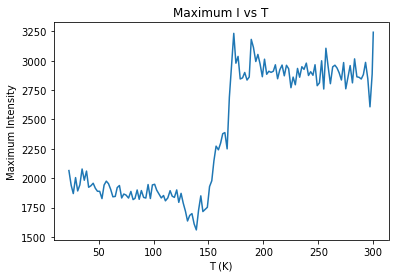
\includegraphics[scale=0.35]{../figs/maxI.png}
  \caption{Maximum intensity value as a function of function temperature.}
  \label{fig:maxI}
\end{figure}

\begin{figure}[h]
\begin{tabular}{ll}
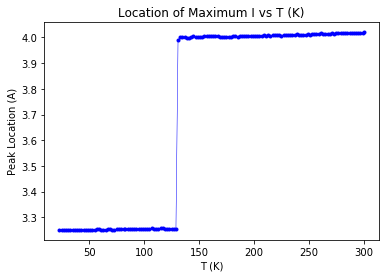
\includegraphics[scale=.4]{../poster/figs/dsmax.png}
&
\hspace{25mm}
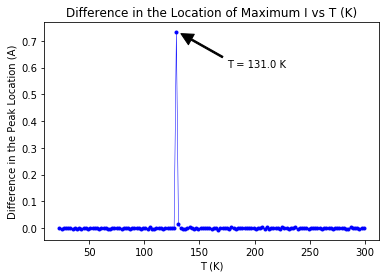
\includegraphics[scale=0.4]{../figs/dsdiff_T.png}
\end{tabular}
\caption{Left: Location of the maximum intensity value as a function of function temperature. 
Right: Difference of maximum intensity value between two adjacent temperatures as a function of function temperature.}
\label{fig:Tmax}
\end{figure}

Besides looking at the maximum intensity, one can also plot the location of the brightest peak as a function of temperature. Figure \ref{fig:Tmax} shows that before the phase transition, the brightest peak is around 3.2 Angstroms but after, the dominant peak is around 4 A. If we plot the difference between the temperatures at T+1 and T we can clearly see where the jump occurred.



\section{The 3.25 $\AA$ Peak } \label{Peak}
	To be able to detect a phase transition we first need to be able to detect a peak and characterize its features. In this section we describe how to characterize a peak. In particular, we will look at the peak located between 3.2 and 3.3 ${\AA}$.
	We characterize a peak by its center, width and area under it. To attribute these values for a given peak, we fit a gaussian function corrected for arbitrary area and background level. The unit area gaussian centered around $x_{0}$ with width $\sigma$ is given by eq. \ref{eq:gaus}
	\begin{equation} \label{eq:gaus}
	f(x) = \frac{1}{\sqrt{2\pi \sigma}} e^{-\frac{(x - x_{0})}{2\sigma^{2}} },
	\end{equation}
	
	We can add a constant background to this function by adding a constant $b$ and by multiplying $f(x)$ by A, we can interpret A as the area under the curve:
	\begin{equation} \label{eq:gausB}
	g(x) = Af(x) + b = \frac{A}{\sqrt{2\pi \sigma}} e^{-\frac{(x - x_{0})}{2\sigma^{2}} } + b,
	\end{equation}
	
	As we will see, this function is not a good hypothesis to fit peaks close to the phase transition temperature. The shape of those peaks are not gaussian at all, and a gaussian description is not adequate. A good way to evaluate how well the adopted function describes the data is to calculate the $\chi^{2}$ of the fit and look at the residues distribution. We are not implementing this analysis here. Mainly because we are actually not interested in the actual value of the area, or width of these peaks, but we are actually interested in finding a way to detect a phase transition. 
	Since the value of these variables will change drastically during a phase transition, this will actually be enough to detect it, so an accurate description of the shape of these peaks is not necessary. By using the function defined in \ref{eq:gausB} we have a very simple interpretation for our data and relatively fast algorithm that scales well with size.
	Figure \ref{fig:fits} shows the fitted curve for T = 0 K and T = 150 K. We can see that far from a phase transition, the fit works fine, whereas close to the phase transition the fit fails. Nonetheless we can see that the fitted values for $A, x_{0} \textrm{ and } \sigma$ are very different which allows us to see something is going on at that temperature.
	Figure \ref{fig:peak3p25} shows the values of $A, x_{0}, \sigma$ and background levels as a function of temperature for the 3.25 $\AA$ peak. Also, we show the same curves normalized in figure \ref{fig:norm} for visualization purposes.
	We can clearly see an interesting structure around 150 K. In all variables, the pattern followed by the curves is drastically changed by this phase transition.
	
	\begin{figure}[h]
	\centering
	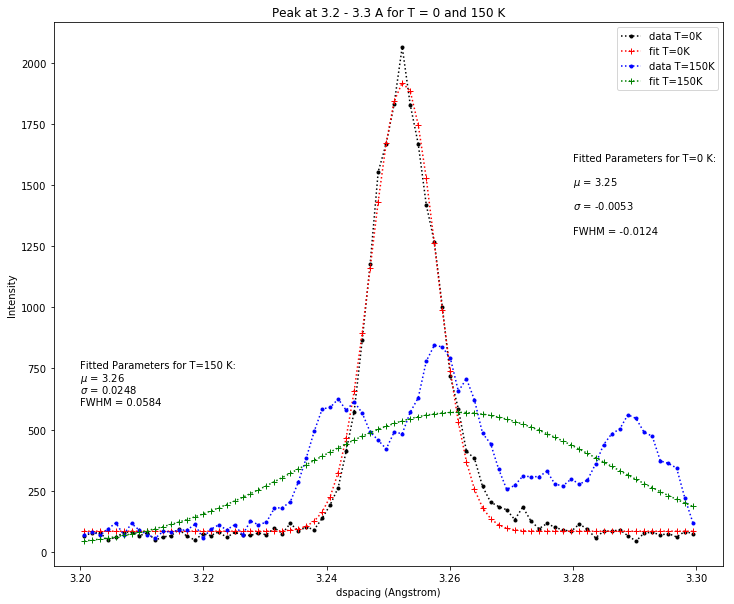
\includegraphics[scale=0.35]{../figs/fits.png}
	\caption{Gaussian fits for T = 0 and 150 K.}
	\label{fig:fits}
	\end{figure}
	
	\begin{figure}[h]
	\centering
	%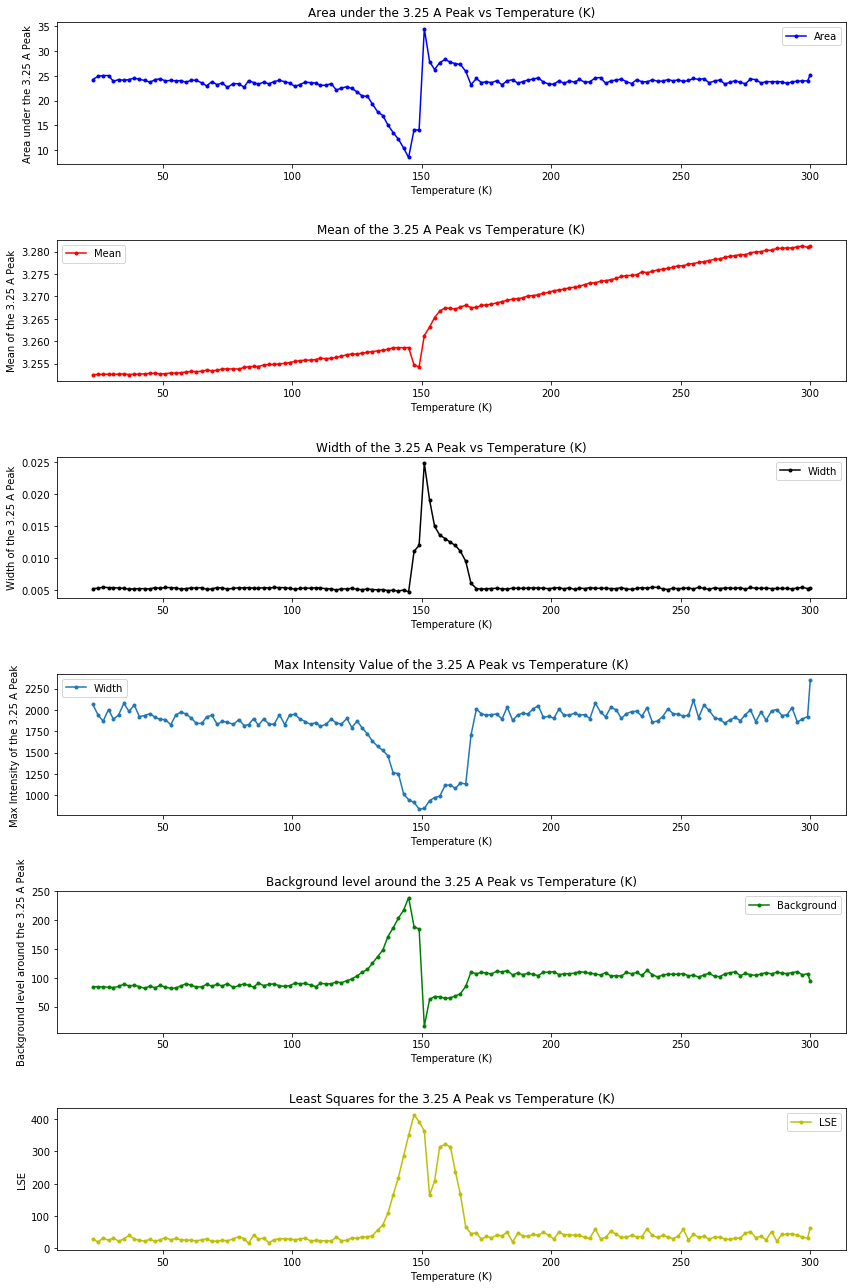
\includegraphics[width=0.8\linewidth, scale=0.25]{../figs/3p25.png}
	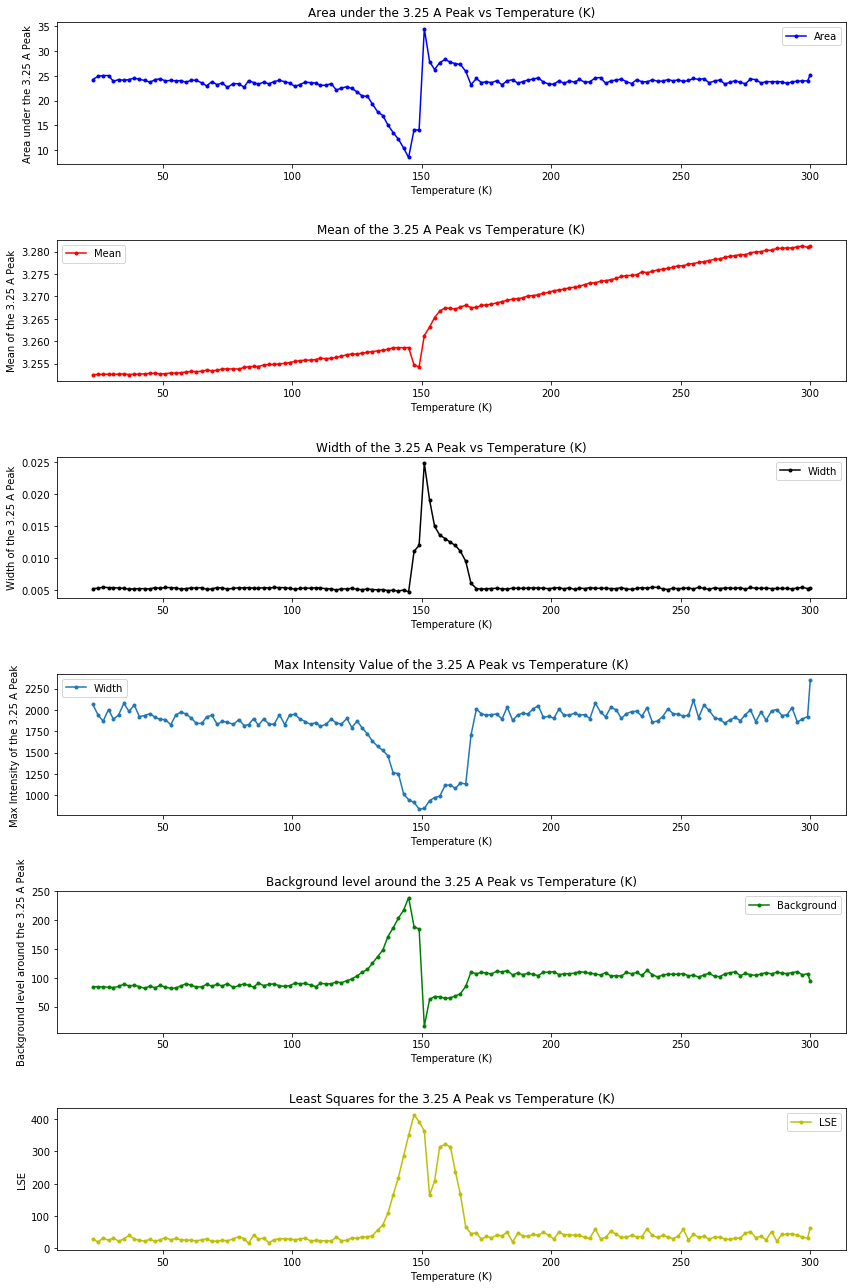
\includegraphics[scale=0.25]{../figs/3p25.png}	
	\caption{Area under the curve, center of the peak, peak width, maximum intensity, background level and chi2 of the fit as a function of temperature.}
	\label{fig:peak3p25}
	\end{figure}

	\begin{figure}[h]
	\centering
	%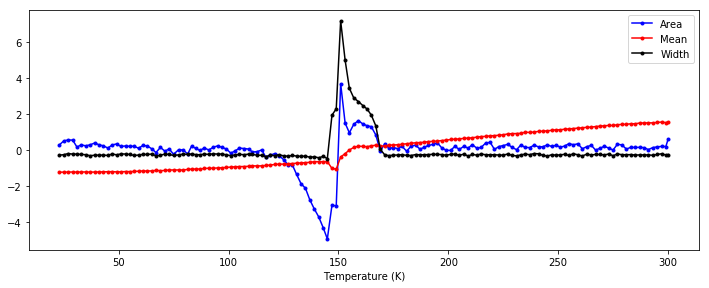
\includegraphics[width=0.8\linewidth]{../figs/norm.png}
	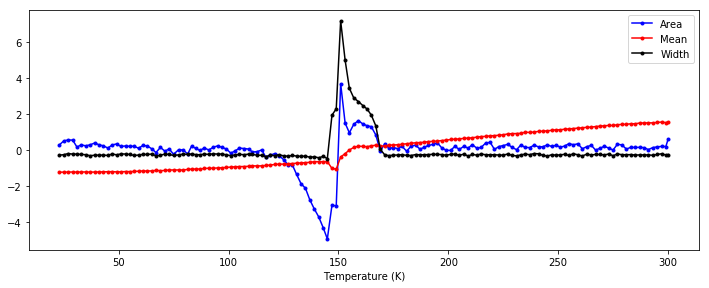
\includegraphics[scale=0.25]{../figs/norm.png}	
	\caption{Normalized area under the curve, center of the peak, peak width and background level as a function of temperature.}
	\label{fig:norm}
	\end{figure}




\section{Finding Peaks} \label{FindPeaks}
	To generalize the procedure of peak characterization we need to be able to detect all the peaks in the data set and study them. To do this, we follow the procedure described in  \cite{DetectPeaks}. We use a simplified form of this algorithm, adapted to our needs and the present data set.
	The way our algorithm works is by declaring all the points in the data set as a possible peak and then start removing peaks that do not satisfy some criteria, namely:
	\begin{enumerate}
  	\item Promote all the data points to peak candidates;
	 \item Remove all the points that are below a certain threshold (defined by the user) - mph;
	 \item Remove all the points that are close to a higher peak, where the distance is defined by the user - mpd;	 
	\end{enumerate}

	Once we detect all the peaks in a data set, we can use the algorithm defined in the previous section (gaussian fit) to construct a list with all the peaks and their variables (number of peaks, areas, centers and widths).
	Figure \ref{fig:findpeaks} shows the detected peaks in the intensity profile for T = 0 K. Ideally we would have systematically tried different values of thresholds for height and distance as described in the algorithm. But in this first study we simply used reasonable values without optimization. A complete optimization of these hyper-parameters is necessary to improve results. But as discussed before, drastic changes in the material structure will still be detected even without further optimization.
	To find the height threshold we first calculate the average intensity of the data set and the standard deviation. We define the threshold as:
	\begin{equation} \label{eq:mph}
	mph = \mu + 1.5\cdot \sigma,
	\end{equation}
	where $\mu$ is the mean value of the data set and $\sigma$, the standard deviation. For the minimum distance we used mpd = 50, i.e, tow peaks have to be at least 50 points apart in the data set.
	
\begin{figure}[h]
  \centering
  %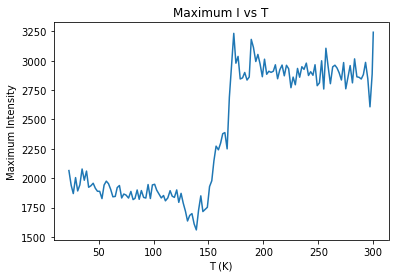
\includegraphics[scale=0.1, width=0.8\linewidth]{../figs/maxI.png}
  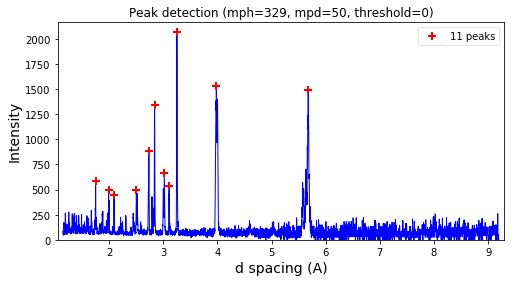
\includegraphics[scale=0.25]{../figs/peaks0.png}
  \caption{Intensity as a function of d-spacing for T = 0 K. The red points indicate the detected peaks in the data.}
  \label{fig:findpeaks}
\end{figure}



\section{Phase Transitions} \label{DefineTransition}
	Finally, we are ready to detect a phase transition in the material. Having an algorithm to find all the peaks in the data and a way to characterize them, we can make a comparison between all the peaks found in two different adjacent temperatures and determine if a phase transition occurred or not.
	Unfortunately, we did not perform a deep study of different ways of detecting a phase transition. In a complete study we can try at least making a peak by peak comparison, but here we propose the following simple criteria:
	\begin{enumerate}
	\item Compare the number of peaks in the two data sets. 
	\item If the number of peaks is different, compare the average width of all the peaks.
	\item A phase transition occurs if: $|w1 - w2| > 0.005$.
	\end{enumerate}
	
	



\section{Conclusions} \label{Conclusions}
	In this study we have defined how to detect a phase transition in a material given intensity data. The process consists of detecting all the peaks in the data for two adjacent temperatures and calculating defining quantities for every peak, namely, their areas, centers and widths.
	For sets with different number of peaks in the data and with different average width (difference $> 0.005$) we declare that a phase transition has occurred.
	
\section{Appendix}\label{App}
	The code used to generate the plots in this study can be found in gcsantucci github repository under SMC DataChallenge Diffraction \cite{git}.
	
\begin{thebibliography}{9}

 \bibitem{DetectPeaks}
 \href{http://nbviewer.jupyter.org/github/demotu/BMC/blob/master/notebooks/DetectPeaks.ipynb}{http://nbviewer.jupyter.org/github/demotu/BMC/blob/master/notebooks/DetectPeaks.ipynb}

 \bibitem{git}
 \href{http://github.com/gcsantucci/SMC_DataChallenge_Diffraction}{http://github.com/gcsantucci/SMC\_DataChallenge\_Diffraction}

\end{thebibliography}
	
\end{document}

